\section{需求基础}

\subsection{需求的定义}
IEEE的需求定义:
\begin{enumerate}[label=(\arabic*)]
    \item 用户为了解决问题或达到某些目标所需要的条件或能力;
    \item 系统或系统部件为了满足合同、标准、规范或其它正式文档所规定的要求而需要具备的条件或能力;
    \item 对(1)或(2)中的一个条件或一种能力的一种文档化表述。
\end{enumerate}

\subsection{基本概念区分}

\subsubsection{问题域}
\begin{itemize}
    \item 问题的产生地:当现实的状况与人们期望的状况产生差距时,就产生了问题。
    \item 要解决问题,就需要改变现实当中某些实体的状态或改变实体状态变化的演进顺序,使其达到期望的状态或演进顺序。
    \item 这些实体和状态构成了问题解决的基本范围,称为该问题的问题域。
\end{itemize}

\subsubsection{解系统}
软件系统通过影响问题域,能够帮助人们解决问题,称之为解系统
\begin{itemize}
    \item 问题域是自治的,它有自己的运行规律,而且这些规律不会因解系统的引入而发生改变
    \item 用户应关注问题域,\textbf{开发者应以问题域为中心思考}
\end{itemize}

\subsubsection{软件解决问题的基础:模拟与共享}
软件系统能够与问题域进行交互和相互影响的原因在于\textbf{软件系统中的某些部分对问题域中的某些部分的具有模拟特性}
\begin{itemize}
    \item 软件系统当中含有问题域某些部分的模型(或模拟),常见的模型包括数据模型、对象模型、处理模型等
    \item 问题域中的某些信息能够和模型中的信息建立映射关系
\end{itemize}
 
这些通过映射建立的共同知识,就是问题域和解系统之间的共享现象
\begin{itemize}
    \item 共享现象就是解 系统所模拟的问题域部分,该部分在两个系统中同时存在
    \item 除了共享现象之外, 同题城还有一些没有被解系统模拟的知识,因为现实世界非常复杂,不可能也没必要在解系统中完全重现 
\end{itemize}
\begin{figure}[H]
	\centering
	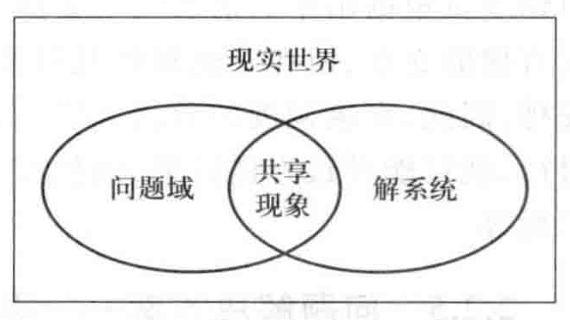
\includegraphics[width=0.3\textwidth]{img/问题域和解系统的关系.png}
\end{figure}

\subsubsection{问题域的特性}
问题域自治的规律性称为问题域特性
\begin{itemize}
    \item 问题域是自治的,它有自己的运行规律,而且这些规律不会因解系统的引入而发生改变
\end{itemize}

需额外关注的问题域特性
\begin{itemize}
    \item 间接特性
    \item 约束和假设 
    \begin{itemize}
        \item 社会性因素
    \end{itemize}
\end{itemize}

问题域特性的重要性
\begin{itemize}
    \item 要想解决问题,它就需要了解问题域特性,将解决方案和问题域特性结合起来 
    \item 要防止解系统的引入在问题域当中引发未预见的连锁反应 (例:间接特性不直接与解系统交互而引发)
\end{itemize}

\subsubsection{解系统的特性}
\begin{itemize}
    \item 解系统是问题的解决手段,并不是问题的产生地,所以解系统并不是问题域的一部分。解系统与问题域之间存在可以互相影响的接口,以实现交互活动。
    \item 用户不应该关注软件系统,而是关注问题。
    \item 开发者关注软件系统,但要学会以问题为中心思考。
\end{itemize}


\begin{figure}[H]
	\centering
	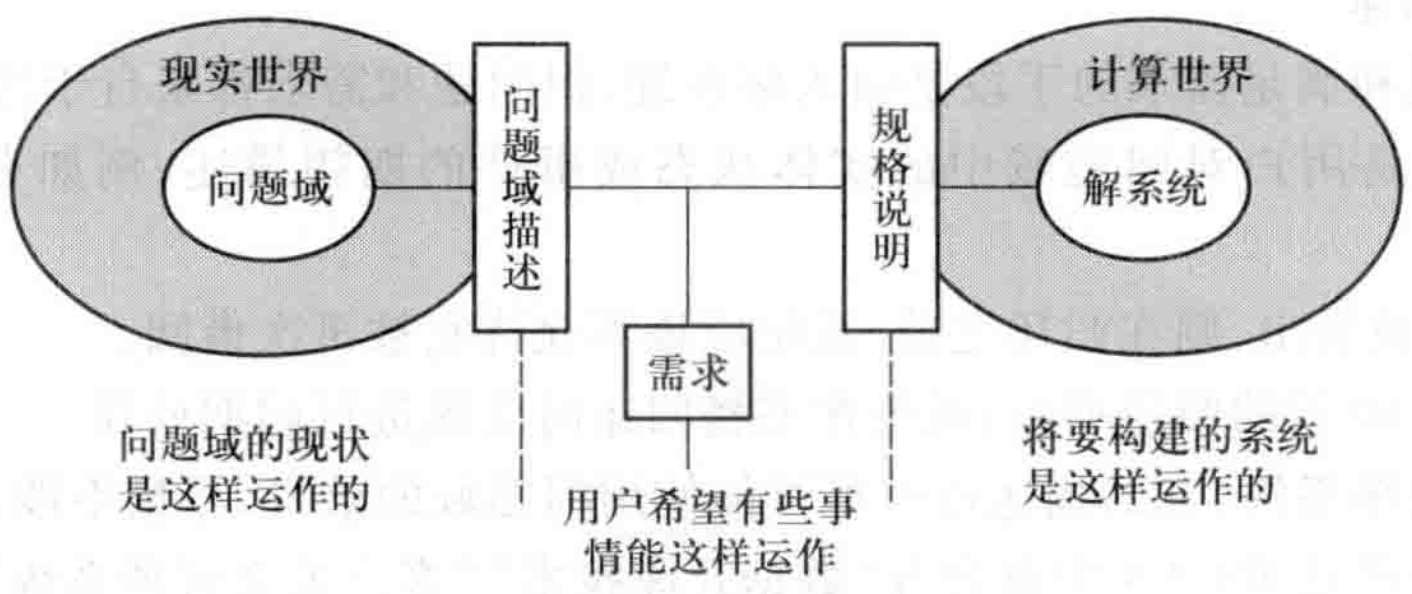
\includegraphics[width=0.55\textwidth]{img/问题域、需求、解系统、需求规格说明关系示意图.png}
\end{figure}

\subsubsection{需求规格说明}
因为解决方案以对外交互的方式定义了软件系统的功能,所以解决方案被称为软件系统的需求规格说明

IEEE将需求规格说明定义为:规定系统或部件的需求的文档,典型地包括功能需求、性能需求、接口需求、设计需求和开发标准。

\subsubsection{需求开发的形式化定义}
描述明确的问题域特性$E$,定义良好的系统行为$S$,预期的需求$R$
\begin{itemize}
    \item 需求工程的目的就是根据$E$,构建$S$,使得$E,S\mapsto R$
    \item 需求工程的困难之处:
    \begin{itemize}
        \item 不存在描述明确的$E$
        \item 不存在确定的针对$S$的评估标准$R$;
        \item $E,S \Rightarrow R$是一个创造性的过程。
    \end{itemize}
    \item 需求工程的主要工作:
    \begin{itemize}
        \item 需求开发,确定$R$
        \item 研究问题背景,描述问题域特性$E$
        \item 构建解系统,描述解系统行为$S$,使得$E,S\mapsto R$
    \end{itemize}
\end{itemize}

\subsubsection{需求工程的基本活动与实质}
\begin{figure}[H]
	\centering
	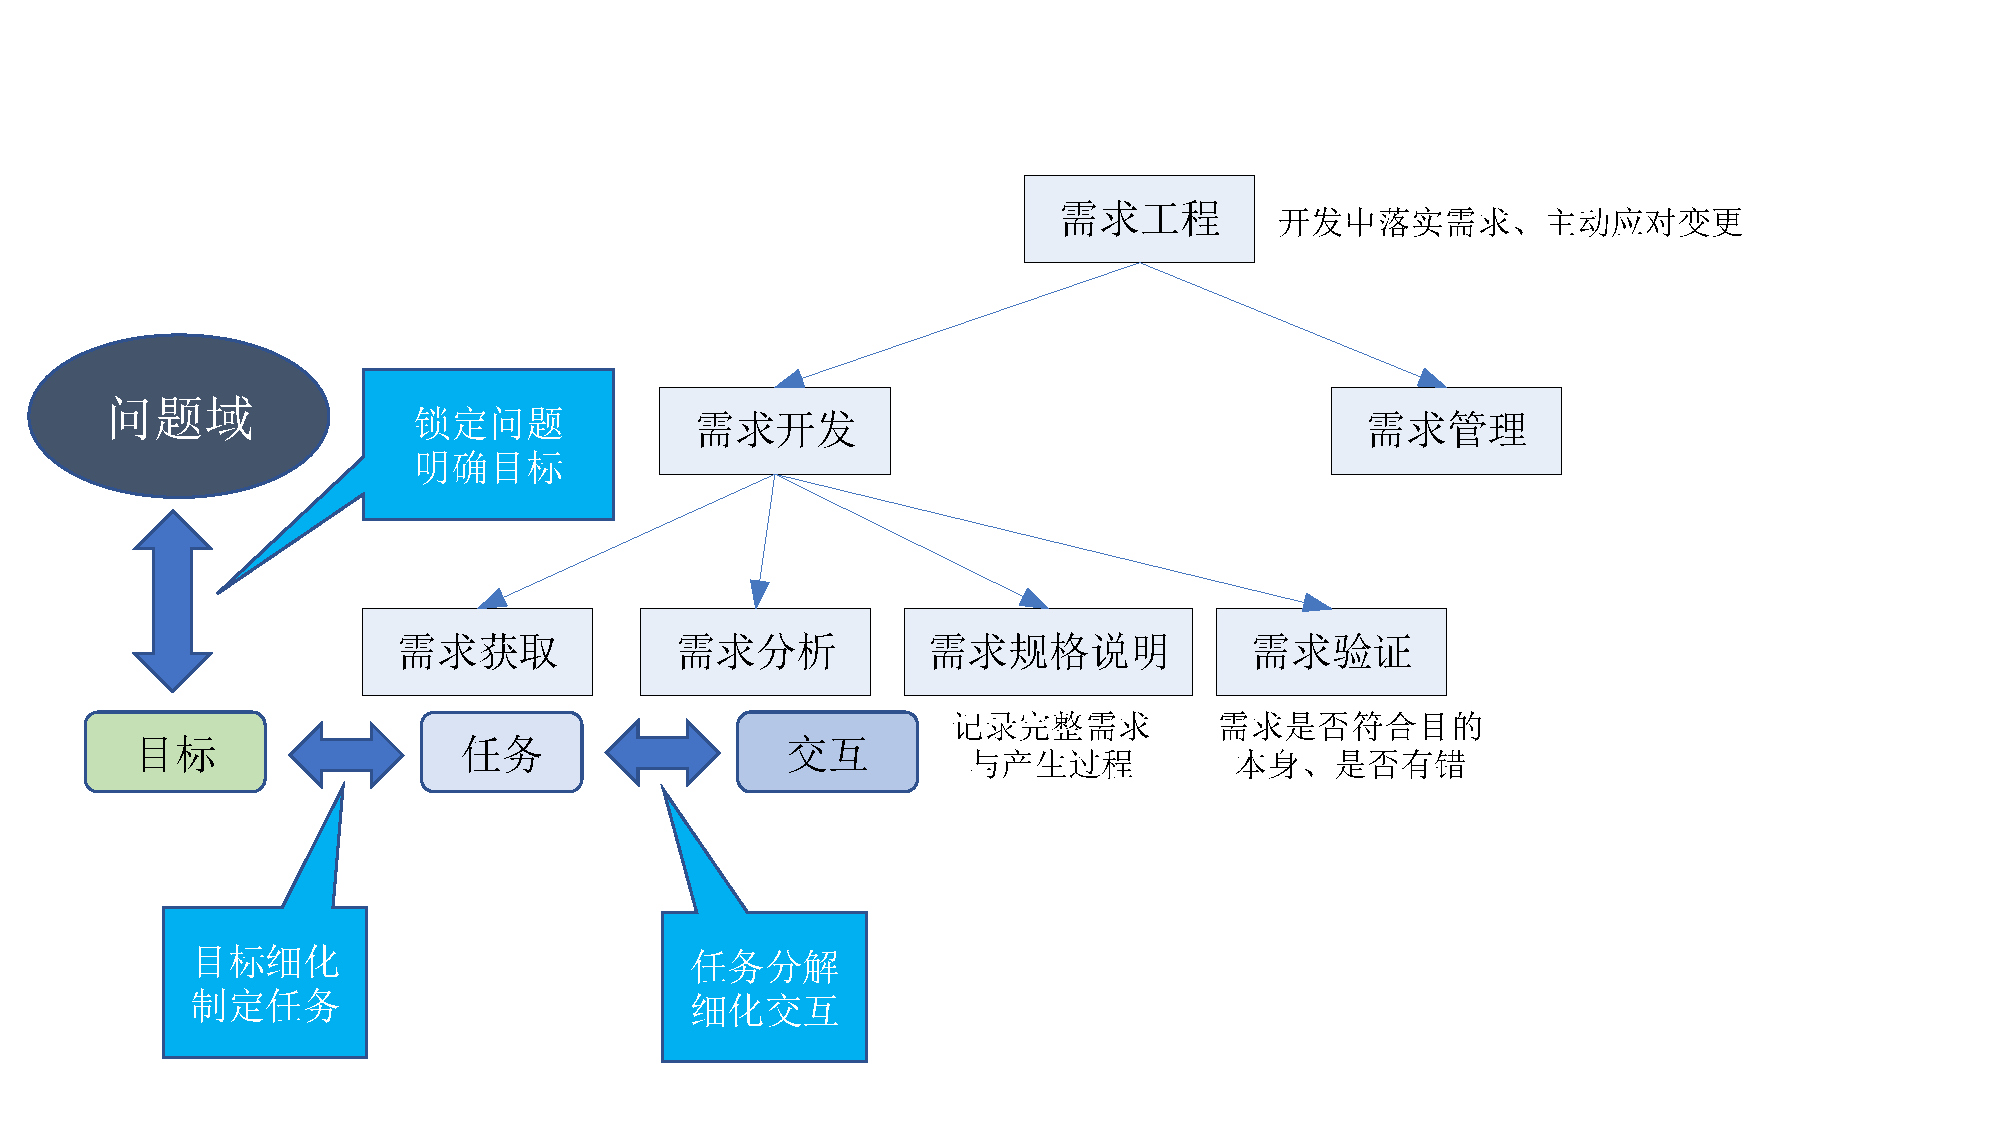
\includegraphics[width=0.8\textwidth]{img/需求工程的基本活动与实质.pdf}
\end{figure}

\subsubsection{需求工程活动的困难性}
\begin{itemize}
    \item 问题域、目标、任务、交互的相互转化是创造性的活动
    \begin{itemize}
        \item 每个案例都有其独特性,不可复用,接近于艺术
        \item 需要对问题所在的领域有着深刻的认识
        \item 需要掌握一套设计思维与辅助工具,并多多练习
    \end{itemize}
    \item 编程与设计方面的能力不能直接用于需求分析 
    \begin{itemize}
        \item 设计和编程都有构建高质量软件的共同目标,而且使用相同的概念和组织机制保证了从设计到编程的平滑过渡,所以,结构化与面向对象思维在设计领域也取得了成功
        \item 但是需求分析除了拥有构建高质量软件的目标之外,还有一个更加重要的目标是理解现实中的非技术性和社会性因素
    \end{itemize}
    \item 文档撰写、功能验证、基线管理需要丰富的开发与管理经验
\end{itemize}


\subsubsection{需求工程师:现实世界方面与技术方面的桥梁}
好的需求工程师更应该扮演好涉众代理的角色,站在涉众的立场想问题,替涉众跟踪和监控软件开发过程,保护涉众的利益
\begin{figure}[H]
	\centering
	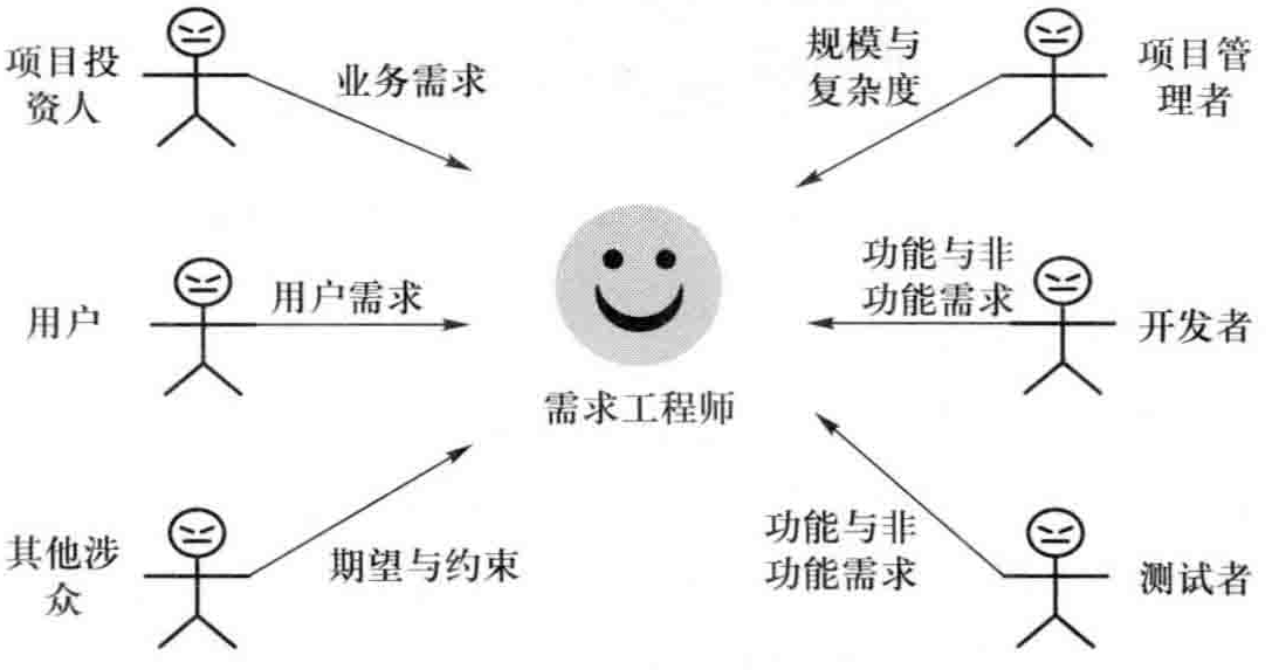
\includegraphics[width=0.6\textwidth]{img/需求工程师的桥梁作用.png}
\end{figure}

需求工程师需要具备的技能
\begin{figure}[H]
	\centering
	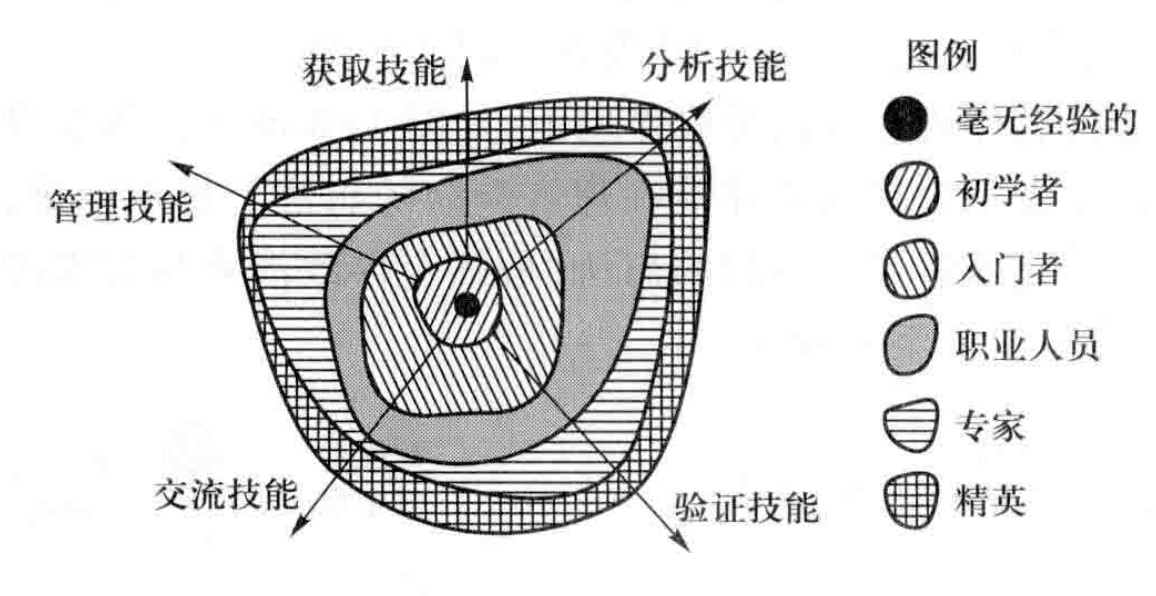
\includegraphics[width=0.55\textwidth]{img/需求工程师需要具备的技能.png}
\end{figure}

\subsection{需求的层次性}
需求是问题解决的期望,问题是可大可小的,期望自然也是可大可小的。问题和期望粒度不同的现象被称为需求的不同抽象层次。

需求最为常见的抽象层次有3层:
\begin{itemize}
    \item 业务需求:针对整个业务的期望,例如:在系统使用3个月后, 销售人员进行销售处理的工作效率应该提高20\%。
    \item 用户需求:针对具体任务的期望,例如:收银员可以使用系统完成销售处理。
    \item 系统级需求:针对用户与系统一次交互的期望,例如:在收银员请求计算已输人商品的总价时,系统应根据规则Rule1($\mbox{总价}=\sum(\mbox{价格}\times \mbox{数量} \times \mbox{折扣})$)计算总价并显示。
\end{itemize}

\begin{figure}[H]
	\centering
	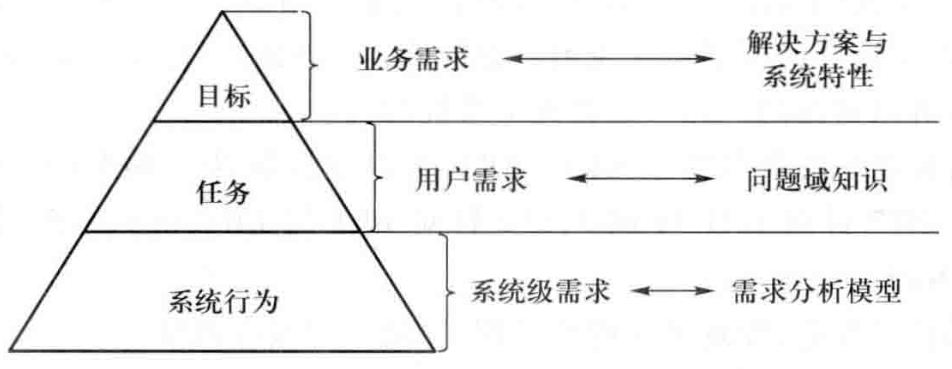
\includegraphics[width=0.55\textwidth]{img/需求的层次性.png}
\end{figure}


\subsubsection{战略问题与业务需求}
业务需求(Business Requirement,BR)是抽象层次最高的需求,是系统建立的战略出发点,表现为高层次的目标,它描述了组织为什么要开发系统。

为了满足用户的业务需求,需求工程师需要描述系统高层次的解决方案(逐一细化),定义系统应该具备的特性(System Feature, SF)
\begin{itemize}
    \item 参与各方必须要对高层次的解决方案达成一致,以建立一个共同的前景
    \item 特性说明了系统为用户提供的各项功能,它限定了系统的范围
    \item 项目的前景和范围明确了软件(某版本)的开发范畴
\end{itemize}

连锁商店销售系统业务需求示例:
\vspace{-0.25em}
{\kaishu \begin{compactitem}
    \item BR1(核心资源):在系统使用6个月后,商品积压、缺货和报废的现象减少50\%。
    \item BR2(关键业务):在系统使用3个月后,销售人员工作效率提高50\%。
    \item BR3(成本结构):在系统使用6个月后,店铺运营成本降低15\%。
    \item BR4(收入来源):在系统使用6个月后,销售额度提高20\%。
\end{compactitem}}

针对业务需求的系统特性:
\vspace{-0.25em}
{\kaishu \begin{compactitem}
    \item SF1:分析店铺商品库存,发现可能的商品积压、缺货和报废现象。BR1,BR3
    \item SF2:根据市场变化调整销售的商品。BR1,BR3,BR4
    \item SF3:制定促销手段,处理积压商品。BR1,BR3,BR4
    \item SF4:与生产厂家联合进行商品促销。BR1,BR3,BR4,CH
    \item SF5:制定促销手段进行销售竞争。BR1,BR4,CH
    \item SF6:掌握员工变动和授权情况。BR2
    \item SF7:处理商品入库与出库。BR1
    \item SF8:发展会员,提高顾客回头率。BR4,CR
    \item SF9:允许积分兑换商品和赠送吸引会员的礼品,提高会员满意度。BR3,BR4,CR
    \item SF10:帮助收银员处理销售与退货任务。BR2
\end{compactitem}}


\subsubsection{任务问题与用户需求}
用户需求是执行实际工作的用户对系统所能完成的具体任务的期望,描述了系统能够帮助用户做些什么。

用户需求是对任务的期望,基本表达方式“$\ast$$\ast$ 用户可以使用系统完成$\ast$$\ast$任务”。
\begin{itemize}
    \item 用户任务应该是有价值的活动(客户洞察),并具有较强的目标性(细化的讲故事与场景)。比如向“ATM机中插卡”就不是用户需求,因为用户不会漫无目的的插卡。
    \item 对所有的用户需求,都应该有充分的问题域知识作为支持。
\end{itemize}

用户需求的特点:
\begin{itemize}
    \item 模糊、不清晰:允许使用形容词和副词 
    \item 多特性混杂:允许混合功能和非功能性需求 
    \item 多逻辑混杂:一条用户需求所代表的任务需多次系统交互才能完成
    \begin{itemize}
        \item 需求开发阶段可视作从用户需要解决的问题到用户与系统的一系列交互的转化,此过程中用户的输入与获得的反馈不断精化,但系统本身仍被视作一个整体,留待后续设计阶段确定模块划分与结构
    \end{itemize}
\end{itemize}

例:在超市管理系统中,收银员用户的需求为:
\vspace{-0.25em}
{\kaishu \begin{compactitem}
    \item UR1:收银员可以使用系统逐一记录销售的商品。
    \item UR2:收银员可以使用系统计算商品账单并处理付款情况,账单计算需要使用促销策略。
    \item UR3:收银员可以使用系统为顾客打印收据。
    \item UR4:收银员可以使用系统退回顾客已经购买的商品。
\end{compactitem}}
  

\subsubsection{系统行为问题与系统级需求}
系统级需求是用户对系统行为的期望,一系列的系统行为联系在一起可以帮助用户完成任务,满足业务需求。

系统需求可以直接映射为系统行为(对应需求规格说明),定义了系统中需要实现的功能,描述了开发人员需要实现什么。

将用户需求转化为系统需求的过程是一个复杂的过程
\begin{itemize}
    \item 首先需要分析问题领域及其特性,从中发现问题域和计算机系统的共享知识,建立系统的知识模型;
    \item 然后将用户需求部署到系统模型当中,即定义系列的系统行为,让它们联合起来实现用户需求,每一个系统行为即为一个系统需求。
    \item 该过程就是需求工程当中最为重要的需求分析活动,又称建模与分析活动。 
\end{itemize}

系统级需求示例如下表所示
\vspace{-0.8em}
\begin{center}
    \begin{longtable}{|m{2cm}|m{11cm}|}
        \hline
        \multicolumn{1}{|c|}{需求ID}    &     \multicolumn{1}{c|}{需求描述}                                                             \\ \hline
        SR1     & 在收银员输入商品目录中已存在的商品标识时,系统显示输入商品的信息,包括ID、名称、描述、价格、特价、数量、总价。ID的规则参见DR1             \\ \hline
        \quad SR1.1   & 在收银员要求输入数量时,系统应该允许收银员输入商品的数量                                                   \\ \hline
        \quad\quad SR1.1.1 & 在收银员输入大于等于1的整数时,系统修改商品的数量为输入值,并更新显示                                            \\ \hline
        \quad\quad SR1.1.2 & 在收银员输入其他内容时,系统提示输入数量无效                                                         \\ \hline
        \quad SR1.2   & 系统应该计算并显示输入商品的总价                                                               \\ \hline
        \quad\quad SR1.2.1 & 如果存在适用(商品标识、今天)的商品特价策略(参见Rule3),系统将该商品的特价设为特价策略的特价,并计算分项总价为(特价$\times$ 数量),并将其计入特价商品总价 \\ \hline
        \quad\quad SR1.2.2 & 在商品是普通商品时,系统计算该商品分项总价为(商品的价格$\times$商品的数量),并将其计入普通商品总价                                \\ \hline
        \quad SR1.3   & 在显示商品信息0.5秒之后,系统显示已输入商品列表,并将新输入商品添加到列表中                                        \\ \hline
        SR2     & 在收银员输入商品目录中不存在的商品标识时,系统不予处理                                                    \\ \hline
        DR1     & ID是规则为……的商品条形码                                                                  \\ \hline
        Rule3   & 适用(商品标识,参照日期)的商品特价促销策略:(促销商品标识$=$商品标识)而且((开始日期早于晚于参照日期)并且(结束日期晚于等于参照日期))         \\ \hline
    \end{longtable}
\end{center}
\vspace{-3.7em}

用户需求和系统级需求在实践中经常是混淆的
\begin{itemize}
    \item 用户习惯于用户需求;
    \item 开发者需要系统级需求,但得到的往往是用户需求
    \begin{itemize}
        \item 未能得到足够信息以准确地完成设计与实现工作
        \item 需要开发者以各自方式进行假设……
    \end{itemize}
\end{itemize}

正确处理用户需求和系统级需求
\begin{itemize}
    \item 明确其不同点
    \vspace{-0.8em}
	\begin{multicols}{2}
    \begin{itemize}
        \item 用户需求:任务
        \item 系统级需求:交互
    \end{itemize}
	\end{multicols}
	\vspace{-1em}
    \item 明确建立和维护用户需求与系统级需求的关系
    \item 系统级需求的建立需要需求分析人员的创造性(建模)
\end{itemize}

\subsection{需求的分类与表述}

\subsubsection{软件需求的分类}
[IEEE 1998]将需求分成下列几个类别:
\begin{itemize}
    \item \textbf{功能需求:}和系统主要工作相关的需求,即在不考虑物理约束的情况下,用户希望系统所能够执行的活动,这些活动可以帮助用户完成任务。功能需求主要表现为系统和环境之间的行为交互。
    \item \textbf{性能需求:}系统整体或系统组成部分应该拥有的性能特征,例如CPU使用率、内存使用率等。
    \item \textbf{质量属性:}系统完成工作的质量,即系统需要在一个“好的程度”上实现功能需求,例如可靠性程度、可维护性程度等。
    \item \textbf{对外接口:}系统和环境中其他系统之间需要建立的接口,包括硬件接口、软件接口、数据库接口等等。
    \item \textbf{约束:}进行系统构造时需要遵守的约束,例如编程语言、硬件设施等。
    \item \textbf{其他:}项目中也可能会出现逻辑数据需求等其他特殊类型的需求。
\end{itemize}

\subsubsection{功能需求}
功能性需求是一个软件产品得以存在的愿意,是软件系统能够解决用户问题和产生价值的基础,也是整个软件开发工作的基础。

通常一个软件系统的绝大部分需求都是功能需求,但在比例上功能需求有可能占所有需求的90\%以上。

在大规模软件系统中,因为其功能需求比较复杂,所以它是最需要按照了个抽象层次进行展开的需求类别,也就是说功能需求的开发要围绕“目标$\rightarrow$任务$\rightarrow$交互”(BR(SF)$\rightarrow$UR$\rightarrow$SR)的路线进行,对“目标”、“任务”和“交互”3个概念的关注是功能需求开发的重中之重。

\subsubsection{性能需求}
[IEEE 1990]对性能的定义是:一个系统或其组成部分在限定的约束下,完成其指定功能的程度,如速度、精确性和内存使用程度等。性能需求定义了系统必须多好和多快地完成专门的功能。

常见的性能需求包括以下几种
\begin{itemize}
    \item 速度(Speed),系统的响应时间。PR1:所有的用户查询都必须在10秒内完成。
    \item 容量(Capacity),系统所能存储的数据量。PR2:系统应该能够存储至少10万条销售记录。
    \item 吞吐量(Throughput),系统在连续的时间内完成的事务数量。PR3:解释器每分钟应该至少解析5000条没有错误的语句。
    \item 负载(Load),系统可以承载的并发工作量。PR4:系统应该允许200个用户同时进行正常的工作。
    \item 实时性(Time-Critical),严格的实时要求。PR5:监测到病人异常后,监控器必须在0.5秒内发出警报。
\end{itemize}

\subsubsection{质量属性}
\begin{itemize}
    \item 系统为了满足规定的及隐含的所有要求而需要具备的要素称为质量(包含性能需求) 
    \item 质量属性是为了度量质量要素而选用的特征 
    \item 质量模型就是能够为质量需求的描述和评价提供工作基础的特征集及特征之间的联系 
\end{itemize}

常见的质量属性示例:
\begin{itemize}
    \item 可靠性(Reliability):在规格时间间隔内和规定条件下,系统或部件执行所要求能力的能力
    \begin{itemize}
        \item QR1:在进行数据的下载和上传中,如果网络故障,系统不能出现故障
        \begin{itemize}
            \item QR1.1:分店子系统应该检测到故障,并尝试重新连接网络3次,每次15秒
        \end{itemize}
    \end{itemize}
    \item 可用性(Availability):软件系统在投入使用时可操作和可访问的程度或能实现其指定系统功能的概率
    \begin{itemize}
        \item QR2:系统的可用性要达到98\%
    \end{itemize}
    \item 安全性(Security):软件阻止对其程序和数据进行未授权访问的能力,未授权的访问可能是有意,也可能是无意的
    \begin{itemize}
        \item QR3:收银员只能查看,不能修改、删除VIP顾客的信息
    \end{itemize}
    \item 可维护性(Maintainability):软件系统或部件能修改以排除故障、改进性能或其他属性或适应变更了的环境的容易程度,包括可修改性(Modifiability)和可扩展性(Extensibility)
    \begin{itemize}
        \item QR4:如果系统要增加新的特价类型,要能够在2个人月内完成。
    \end{itemize}
    \item 可移植性(Portability):可移植性指系统或部件能从一种硬件或软件环境转换至另外一种环境的特性
    \begin{itemize}
        \item QR5:服务器要能够在1人月内从Windows7操作系统更换到Solaris 10操作系统。
    \end{itemize}
    \item 易用性(Usability):与用户使用软件所花费的努力及其对使用的评价相关的特性。
    \begin{itemize}
        \item QR6:使用系统1个月的收银员进行销售处理的效率要达到10件商品每分钟
    \end{itemize}
\end{itemize}

\begin{figure}[H]
	\centering
	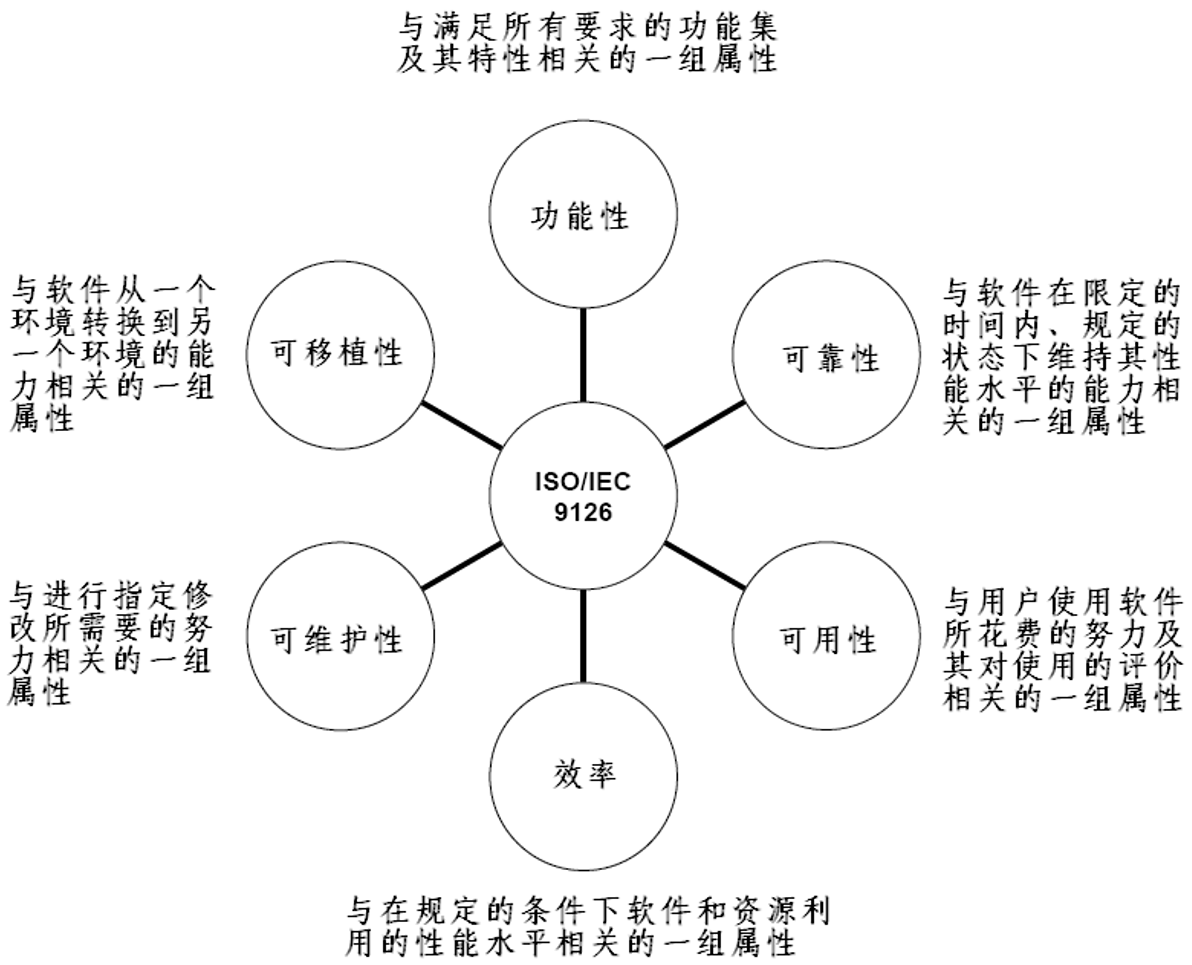
\includegraphics[width=0.6\textwidth]{img/质量属性举例.png}
\end{figure}

\subsubsection{对外接口}
对系统之间的软硬件接口需要说明以下内容
\vspace{-0.8em}
\begin{multicols}{3}
\begin{itemize}
    \item 接口的用途
    \item 接口的输入输出
    \item 数据格式
    \item 命令格式
    \item 异常处理要求
\end{itemize}
\end{multicols}
\vspace{-1em}

对外接口需求规格片段
{\kaishu 
\vspace{-0.8em}
\begin{multicols}{2}
    \columnseprule=0.8pt
    IR1:与地图API的接口:定位用户与商户的位置 \\
    参数:手机GPS定位坐标。\\
    返回值:在地图的定位,并基于此给出最近的商家。
    
    IR2:支付宝接口:订单生效应允许通过支付宝付款。\\
    参数:商家支付宝号,顾客支付宝号,应付款额。\\
    返回值:支付成功或支付失败状态。
\end{multicols}
\vspace{-1em}}

用户界面在有些情况下也会被视为系统的对外接口,被作为一种重要的需求。但[CMU/SEI1991]认为,和其他需求相比,用户的界面更经常发生变化,进而影响需求的稳定性,所以[CMU/SEI1991]建议如果将用户界面作为需求一部分的话,一定要进行单独处理和组织。通常,对于人机交互复杂的系统使用单独的人机交互设计文档记录用户界面需求,否则可以将其作为需求文档的一部分进行记录。

\subsubsection{约束}
总体上限制了开发人员设计和构建系统时的选择范围 
\begin{itemize}
    \item 系统开发及运行的环境:包括目标机器、操作系统、网络环境、编程语言、数据库管理系统等
    \item 问题域内的相关标准(商业模式评估):包括法律法规、行业协定、企业规章等
    \item 商业规则(商业模式设计):用户在任务执行中的一些潜在规则也会限制开发人员设计和构建系统的选择范围
\end{itemize}

进入21世纪以来,基于web的产品发展,软件对周围环境的要求越来越突出,尤其是:
\begin{itemize}
    \item 商业规则:目标、规则、边界值与异常情况处理
    \item 法规与行业规范:新业务与灰色地带,利用违规内容抹黑竞争对手
    \item 社会性因素:宗教信仰、价值取向、流行风潮等
\end{itemize}

规则描述样式与示例
\vspace{-0.8em}
\begin{center}
    \begin{longtable}{|m{0.8cm}<{\centering}|m{6.5cm}|m{6.5cm}|}
        \hline
        \multicolumn{1}{|c|}{类别}    &     \multicolumn{1}{c|}{描述样式}    &    \multicolumn{1}{c|}{示例}                                                   \\ \hline
        术语                  & {[}限定词{]}\textless{}名词/业务术语\textgreater{}是指\textless{}文字描述\textgreater{}                                                            & Rule2:退货是指顾客在一个时间点上凭之前1周内的购物发票,退回其中一项或多项商品的行为;                        \\ \hline
        \multirow{2}{*}{事实} & {[}限定词{]}\textless{}名词/业务术语1\textgreater{}{[}条件限定{]}必须|可能\textless{}动词或动词短语\textgreater{}{[}限定词{]}\textless{}名词/业务术语2\textgreater{} & Rule3:同样的商品在不同的时期内可能有不同的价格;                                           \\ \cline{2-3} 
                            & \textless{}名词/业务术语1\textgreater{}的特征有\textless{}名词/业务术语2\textgreater{}                                                              & Rule4:每件商品都有一个条形码                                                     \\ \hline
        \multirow{2}{*}{约束} & {[}限定词{]}\textless{}名词/业务术语\textgreater{}必须满足\textless{}条件\textgreater{}                                                            & Rule5:商品条形码符合EAN-13标准                                                 \\ \cline{2-3} 
                            & \textless{}名词/业务术语\textgreater{}必须/不能\textless{}动词或动词短语\textgreater{}\textless{}条件\textgreater{}                                    & Rule6:商品特价的折扣率不能超过50\%                                                \\ \hline
        推导                  & \textless{}名词/业务术语\textgreater{}的计算方式为\textless{}数学计算表达式\textgreater{}                                                              & Rule7:普通商品项总价 = 价格×数量                                                 \\ \hline
        推理                  & 如果\textless{}条件1\textgreater{}{[}和/或者\textless{}条件2\textgreater{}…{]},那么\textless{}结论\textgreater{}                                 & Rule8:如果销售日期在一周之前,或者销售是用积分付款的,或者销售的非积分付款余额已经不足以支付商品退款额,那么该商品就属于不可退货商品 \\ \hline
    \end{longtable}
\end{center}
\vspace{-3.7em}

\subsubsection{其他需求}
\begin{itemize}
    \item 安装需求(例如OR1)、培训需求(OR2)、数据需求等
    
    {\kaishu 
    OR1:在安装系统时,要初始化用户、商品库存等重要数据。\\
    OR2:系统投入使用时,需要对用户进行1个星期的集中培训。
    }
    \item 如果在功能需求中没有描述数据内容(例如SR3),就需要补充描述数据信息(例如DR1$\sim$DR2)。
    
    {\kaishu
    SR3:在收银员输入商品标识时,系统显示商品信息,商品信息参见DR1、DR2;\\
    DR1:ID是规则为……的商品条形码;\\
    DR2:商品信息包括:ID、名称、描述、价格、特价、数量、总价
    }
\end{itemize}

